\chapter*{Introduction: Between Particle and Vibration}
\addcontentsline{toc}{chapter}{Introduction: Between Particle and Vibration}
\markboth{Introduction: Between Particle and Vibration}{Introduction: Between Particle and Vibration}
\vspace{0.6cm}
\begin{center}
\nopagebreak
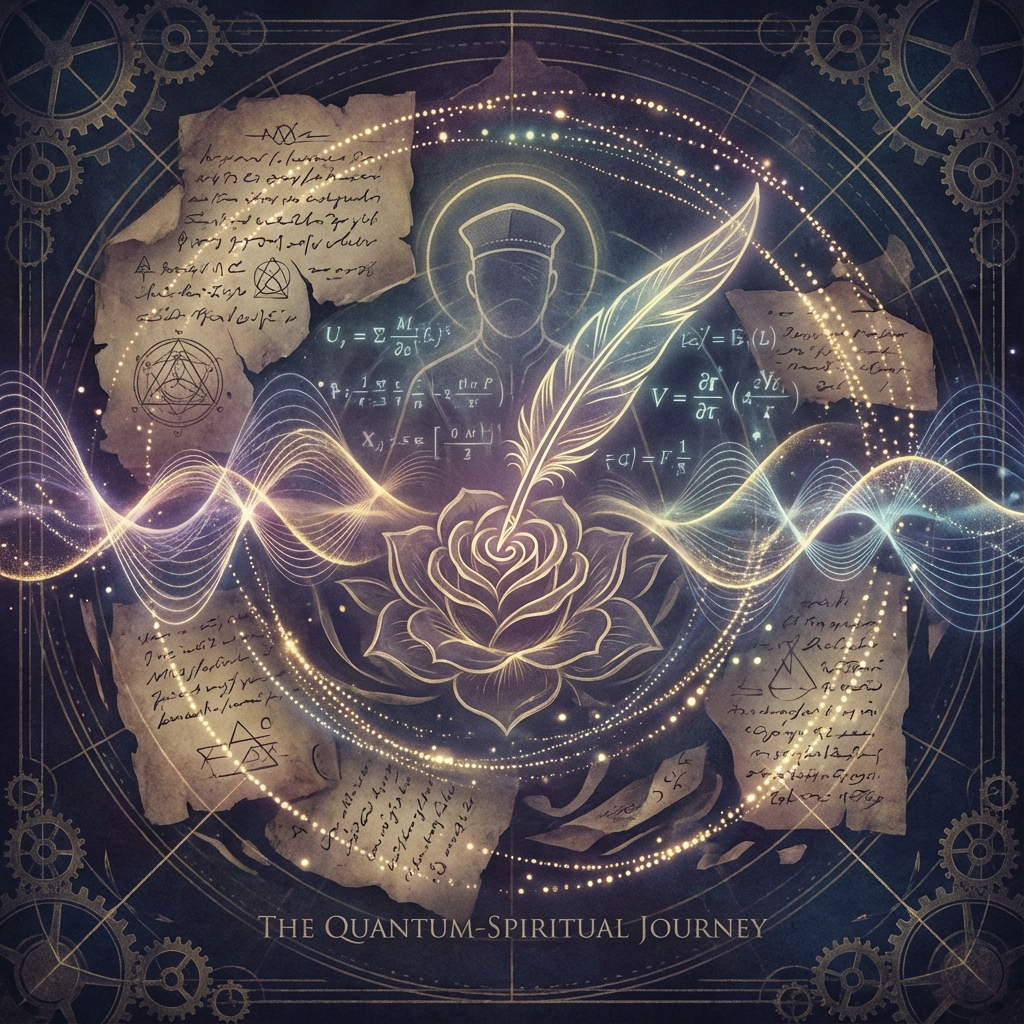
\includegraphics[width=0.75\textwidth,cfbox=gray!60 0.6pt 4pt]{intro_quantum_luther.png}\\
\vspace{4pt}
{\small\itshape Between particle and vibration: the awakening of consciousness.}
\end{center}

\vspace{0.6cm}
I. The Soul's Unrest
For as long as I can remember, I have felt a kind of dissonant vibration whenever I approached the great temples of stone. It wasn't a lack of faith; on the contrary, I have always sensed that behind the veil of reality exists an inexhaustible Source of love. My conflict, my silent torment, was born from the contrast between that intuition of an infinite God and the smallness of the boxes into which we tried to fit Him.


I grew up in the heart of Catholicism, breathing the incense and admiring the liturgy, but very soon, that beauty was clouded by an uncomfortable sensation: pride. It pained my soul to hear, implicitly or explicitly, that we had ``the truth'' and others did not. How could it be that the Creator of a universe of a hundred billion galaxies had a preference for a specific spiritual zip code? I felt we were guilty of a terrible arrogance by not recognizing salvation for other creeds, by looking with pity or superiority at those who sought the light by another path. That exclusivity seemed to me, paradoxically, the most irreligious act of all: limiting God's mercy to our own human borders.


II. The Shadows in the Centers of Power
But my torment went beyond theology. Studying history, I ran into blood-stained walls. The Inquisition, the crusades, the excommunications... I couldn't help thinking: How have we gone from ``love your neighbor'' to ``burn him if he doesn't think like you''?


For years, this pushed me away. I felt rage. I saw the institution and saw only the shadows. However, with time and maturity, I understood something fundamental: the Church, like any human structure, is composed of people. And people are antennas. When fear settles in the centers of power, when the need for control exceeds the need to serve, the collective vibration descends.


The Inquisition was not the work of God, nor was it even the work of ``religion'' in the abstract. It was the inevitable consequence of a \textbf{low vibration} installed at the top. The fear of losing power, the fear of the different, hatred disguised as zeal... all those are dense, heavy frequencies. And when that density takes over a hierarchy, the result is suffering. Obviously, it is something that Christ himself, my friend Jesus, would never have allowed. He, who stopped the stones against the adulteress, would never have lit a bonfire.


Understanding this allowed me to forgive. I understood that it wasn't ``the Church'' that failed, but the vibration of the men who, in dark moments, led it. And that, below that dome of power, there were always thousands of priests, nuns, and laypeople vibrating high, feeding the hungry, comforting the sad, keeping the light burning despite the darkness of their leaders.


III. The Quantum Physics of the Spirit
My definitive reconciliation came from science. I have always been fascinated by quantum physics, that branch of knowledge that tells us that reality is not as solid as it seems. It teaches us that every subatomic particle is, at the same time, matter and wave. It is something concrete and, at the same time, it is pure vibration, pure possibility.


That's where everything clicked. The Lord's Prayer, the teachings of Jesus... they weren't rigid moral rules, they were quantum physics instructions!


When Jesus tells us ``fear not,'' he is not giving us a psychological order, he is telling us: ``Do not lower your frequency.'' Fear is a slow, dense vibration that contracts reality. Love, peace, security... are fast, expansive vibrations that create light.


I understood that ``falling into temptation'' is not eating a cake during Lent. It is the temptation to be dragged down by the gravity of low vibrations: hatred, revenge, envy, pride. When you hate, you become dense. You become a heavy ``particle,'' isolated, disconnected from the whole. When you love, you become a ``wave,'' you expand, you connect with the universal quantum field, with the Father.


IV. A Coffee with Luther
On this journey of understanding, I have often imagined having a coffee with Martin Luther in the 16th century. I think we would have been good friends. He saw that same pride that tormented me. He saw how the structure had become so dense, so concerned with selling indulgences and building marble basilicas, that it had forgotten the vibration of the Gospel.


Luther had the courage to say: ``Salvation is not in Rome, it is in your faith.'' And I would add, from my 21st-century perspective: ``Salvation does not depend on following the Pope, but on the frequency of your heart.''


If your works, if your daily life, are done from the high vibration of love, there is no doubt that you are saved. Because ``being saved'' is not a ticket to join a VIP club after you die. Being saved is living, here and now, in the frequency of Paradise. It is being in tune with the Source.


If a Buddhist, an atheist, or a Christian vibrates in unconditional love, they are on the same frequency. They are ``in God.'' And no bull, no decree, can change that physical and spiritual reality. Salvation is a matter of resonance, not bureaucracy.


V. The Light that Prevails
That is why I am writing this book. Not to attack religion, but to rescue its vibrational essence. I write from love, having healed that pity I felt for institutional pride. I have stopped looking at the darkness of the Inquisition to look at the light of the mystics, of the anonymous saints, of the good people who, in the name of that same faith, have vibrated so high that they have changed the world.


This book is an invitation to walk with Jesus, not as a severe judge, but as a master of vibration. A friend who teaches us to navigate between Madrid, Las Rozas and Colmenarejo without losing the tune. A guide who reminds us, again and again, that we are light, that we are waves, and that our only duty is to keep the frequency high, no matter what happens around us.


So, dear reader, forget for a moment the dogmas, the guilts, and the inherited fears. Open your mind to the possibility that everything, absolutely everything, is music. And that you have the instrument in your hands to play the most beautiful melody.


Welcome to ``My friend Jesus Christ.''